\chapter{Tecnologia}
\section{Introduccion}
El principal elemento de estructura activa de la Capa de Tecnología es el nodo. Este elemento se utiliza para modelar entidades estructurales en esta capa. Modela estrictamente el aspecto estructural de un sistema: su comportamiento está modelado por una relación explícita con el elemento de comportamiento. Una interfaz de tecnología es el lugar (lógico) en el que se puede acceder a los servicios tecnológicos ofrecidos por un nodo mediante otros nodos o mediante componentes de aplicación de la Capa de Aplicación. Los nodos vienen en varias presentaciones, incluyendo software de dispositivos y sistemas. Un dispositivo modela un recurso físico computacional, sobre el cual se pueden desplegar artefactos para su ejecución. El software de sistema es un componente de software de infraestructura que se ejecuta en un dispositivo. Típicamente, un nodo consiste en un número de subnodos; por ejemplo, un dispositivo como un servidor y software de sistema para modelar el sistema operativo.
Las interrelaciones de los componentes de la Capa de Tecnología están formadas principalmente por la infraestructura de comunicación. La trayectoria modela la relación entre dos o más nodos, a través de la cual estos nodos pueden intercambiar información. La realización física de un trayecto se modela con una red de comunicación; es decir, un medio de comunicación físico entre dos o más dispositivos (u otras redes).

\begin{itemize}
	\item Un nodo representa un recurso computacional o físico que alberga, manipula o interactúa con otros recursos computacionales o físicos.
	\item Un dispositivo es un recurso físico TI en el que se pueden almacenar o desplegar programas y artefactos del sistema para su ejecución.
	\item El software del sistema representa el software que proporciona o contribuye a un entorno para almacenar, ejecutar y utilizar el software o los datos desplegados en él.
	\item Una colaboración tecnológica representa un agregado de dos o más nodos que trabajan juntos para realizar un comportamiento tecnológico colectivo.
	\item Una interfaz tecnológica representa un punto de acceso donde los servicios tecnológicos ofrecidos por un nodo
	se puede acceder.
	\item Una red de comunicaciones representa un conjunto de estructuras que conectan sistemas informáticos u otros dispositivos electrónicos para la transmisión, el enrutamiento y la recepción de datos.
\end{itemize}

%\newpage

\section{Metamodelo}
\begin{figure}[h!]
	\centering
	\includegraphics[width=0.9\linewidth]{imgs/meta/Tecnologia}
	\caption{Metamodelo Tecnologia}
	\label{fig:mTech}
\end{figure}

La figura \ref{fig:mTech} da una visión general de los elementos de la Capa de Tecnología y sus relaciones. Siempre que sea aplicable, la concepción se extrae de la analogía con las Capas de Negocio y Aplicación. La Capa de Tecnología se utiliza típicamente para modelar la arquitectura tecnológica de la empresa, definida por el marco TOGAF como: "la estructura e interacción de los servicios de la plataforma, y los componentes tecnológicos lógicos y físicos".

\newpage
\section{Punto de Vista de Implementacion y Despliegue}

El punto de vista de la implementación y el despliegue muestra cómo se realizan una o más aplicaciones en la infraestructura. Esto comprende la asignación de las aplicaciones y componentes a los artefactos, y la asignación de la información utilizada por esas aplicaciones y componentes a la infraestructura de almacenamiento subyacente.\\

Un artefacto representa un dato que se utiliza o se produce en un proceso de desarrollo de software, o por el despliegue y funcionamiento de un sistema informático. Un artefacto representa un elemento tangible en el mundo de la informática. El artefacto es una especialización del objeto tecnológico. Se suele utilizar para modelar productos (software) como archivos de origen, ejecutables, scripts, tablas de bases de datos, mensajes, documentos, especificaciones y archivos modelo. Una instancia (copia) de un artefacto puede ser desplegada en un nodo. Un artefacto puede utilizarse para representar un componente de datos físicos que realiza un objeto de datos.\\

Un componente de aplicación o software de sistema puede ser realizado por uno o más artefactos. Un objeto de datos puede ser realizado por uno o más artefactos. Se puede asignar un nodo a un artefacto para modelar que el artefacto está desplegado en el nodo. Así pues, las dos formas típicas de utilizar el elemento del artefacto son como componente de ejecución o como fichero de datos. De hecho, éstas podrían definirse como especializaciones del elemento del artefacto.
El nombre de un artefacto debe ser preferentemente el nombre del archivo que representa; por ejemplo, orden.jar. Un artefacto puede consistir en sub artefactos.

\clearpage

\subsection{Modelo de Implementacion y Despliegue}
\begin{figure}[h!]
	\centering
	\includegraphics[width=.7\linewidth]{imgs/modelo/Implementacion}
	\caption{Modelo Implementacion y Despliegue}
\end{figure}

Un objeto tecnológico modela los elementos de la estructura pasiva que son utilizados y procesados por la infraestructura. Un artefacto es una pieza física de información que se utiliza o se produce en un proceso de desarrollo de software, o por el despliegue y funcionamiento de un sistema. Es la representación, en forma de, por ejemplo, un archivo, de un objeto de datos o un componente de aplicación, y puede desplegarse en un nodo. El elemento del artefacto se ha tomado de UML. Un objeto tecnológico representa un elemento pasivo que es usado o producido por el comportamiento tecnológico. Los objetos tecnológicos representan los objetos "físicos" manipulados por la infraestructura de una empresa. Los objetos tecnológicos son elementos abstractos, es decir, no están instanciados en modelos sino que sirven como el tipo genérico de las cosas manipuladas por la Capa de Tecnología. Esto puede incluir tanto artefactos (por ejemplo, archivos) como material físico.
Se puede acceder a los objetos tecnológicos por medio del comportamiento tecnológico (funciones, procesos, interacciones, eventos y servicios). Un objeto tecnológico puede tener relaciones de asociación, especialización, agregación o composición con otros objetos tecnológicos. Un objeto tecnológico puede realizar un objeto de datos o un objeto de negocios. Puede realizarse mediante un artefacto o material (de los elementos físicos). El nombre de un objeto tecnológico debe ser preferentemente un sustantivo.

\newpage

\subsection{Caso  de Implementacion y Despliegue}
\begin{figure}[h!]
	\centering
	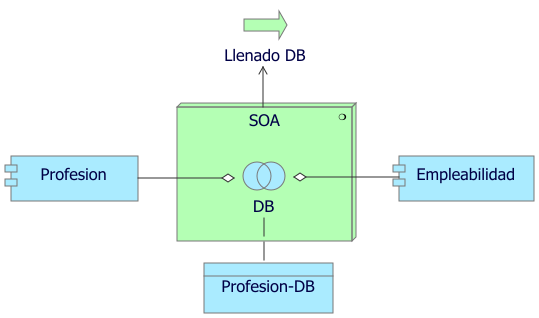
\includegraphics[width=.7\linewidth]{imgs/puntos_vista/tecnologia/despliegue.pdf}
	\caption{Caso Implementacion y Despliegue}
\end{figure}

El proceso tecnológico referente al llenado de la base de datos, corresponde a una colaboración entre el componente de la aplicación Profesión y el componente externo Empleabilidad, dando como resultado la base datos de profesiones con mayor demanda en el ámbito local y fuente estadística para el posterior perfilamiento del componente Estudiante. Asimismo, se visualiza el sistema de software modelado mediante una arquitectura orientada a servicios, que facultará ese proceso tecnológico de llenado de la base de datos. En la capa de aplicación, desarrollamos una arquitectura de orquestación que permitió el modelamiento de componentes, ahora mediante la capa tecnológica y elementos tecnológicos distribuidos específicamente, además de controlar el flujo entre los componentes gracias a la arquitectura de orquestación, podemos agregar elementos externos a nuestro modelo de aplicación local.
\newpage
\subsection{Punto de Vista de la Tecnología}
El punto de vista de infraestructura general, trata acerca del hardware y la infraestructura de comunicación que soporta la capa de aplicación. Esta capa ofrece servicios de infraestructura requeridos para desplegar las aplicaciones realizadas en los ordenadores y los sistemas de
hardware y software.



\subsubsection{Punto de vista de uso de infraestructura}

El punto de vista de uso de infraestructura muestra como las aplicaciones son soportadas por la infraestructura de software y hardware: los servicios de infraestructura son entregados por los dispositivos, los sistemas de software y redes son entregados a las aplicaciones. Este
punto de vista juega un rol importante en el análisis del rendimiento y la escalabilidad y puede ser usado para determinar requerimientos de rendimiento y calidad en la infraestructura basado en las demandas de las aplicaciones que la usan.
\newpage

\begin{figure}[h]
	\centering
	\fcolorbox{black}{white}{
		\includegraphics[width=0.5\linewidth]{imgs/puntos_vista/tecnologia/MMDUDI.jpg}}
	\caption{Metamodelo de uso de infraestructura}
\end{figure}

\subsubsection{Modelo de uso de infraestructura}

En este punto de vista se identifican los servicios de infraestructura principales que corresponden al servicio de notificaciones, generar reportes, establecer tiempos de acceso a la
aplicación, y gestionar los usuarios. Cada uno de los servicios de infraestructura entrega configuración y la funcionalidad requerida hacia los componentes de aplicación.


\begin{figure}[h]
	\centering
	\fcolorbox{black}{white}{
		\includegraphics[width=0.5\linewidth]{imgs/puntos_vista/tecnologia/MDUDI.jpg}}
	\caption{Modelo de uso de infraestructura}
\end{figure}



\subsubsection{ Punto de vista de Implementación y despliegue}
El punto de vista de implementación y despliegue muestra como uno o más aplicaciones son realizadas sobre la infraestructura. Esto implica el mapeo de aplicaciones (lógicas) y componentes en artefactos (físicos). Esta vista juega un papel importante en el análisis del rendimiento y la escalabilidad debido a la relación entre la infraestructura y el mundo lógico de las aplicaciones.


\begin{figure}[h]
	\centering
	\fcolorbox{black}{white}{
		\includegraphics[width=0.5\linewidth]{imgs/puntos_vista/tecnologia/MMDIYD.jpg}}
	\caption{Metamodelo de implementación y despliegue}
\end{figure}

\subsubsection{Modelo de implementación y despliegue}

En este punto de vista, se muestra como todos los componentes son realizados por el nodo de servidor de aplicaciones, el componente de comunicación va a ser realizado por el nodo servidor de aplicaciones y tiene una relación de asociación con el nodo servidor de e-mail que
proveerá las configuraciones de software específico para el envío de notificaciones, resultados e información sobre el proceso.

\begin{figure}[h]
	\centering
	\fcolorbox{black}{white}{
		\includegraphics[width=0.5\linewidth]{imgs/puntos_vista/tecnologia/MDIYD.jpg}}
	\caption{Modelo de implementación y despliegue}
\end{figure}



\begin{table}[h]
	\begin{center}
		\begin{tabular}{ | m{7em} | m{8cm}|  } 
			\hline
			Interesados & Arquitectos de infraestructura, gerentes operativos 
			\\
			\hline
			Preocupaciones & Estabilidad, seguridad, dependencias, costos de la infraestructura
			\\
			\hline
			Propósito & Diseñar
			\\
			\hline
			Alcance & Una capa / aspecto múltiple
			\\
			\hline
		\end{tabular}
		\caption{Punto de Vista Tecnología}
		\label{tab:concepts}
	\end{center}
\end{table}

\textbf{Elementos que participan: }
\begin{itemize}
	\item Ubicación
	\item Nodo
	\item Colaboración tecnológica
	\item Dispositivo
	\item Software del sistema
	\item Interfaz tecnológica
	\item Red de comunicacion
	\item Camino
	\item Proceso tecnológico / función / interacción
	\item Servicio de tecnología
	\item Evento tecnológico
	\item Artefacto
\end{itemize}
\newpage
\section{Punto de Vista de Uso de Tecnología}

El punto de vista de la utilización de la tecnología muestra cómo las aplicaciones son apoyadas por la tecnología de software y hardware: los servicios tecnológicos son suministrados por los dispositivos; el software y las redes del sistema son suministrados a las aplicaciones. Este punto de vista desempeña un papel importante en el análisis del rendimiento y la escalabilidad, ya que relaciona la infraestructura física con el mundo lógico de las aplicaciones. Es muy útil para determinar los requisitos de rendimiento y calidad de la infraestructura en función de las exigencias de las diversas aplicaciones que la utilizan.

\subsection{Modelo de Uso de la Tecnología}
\begin{figure}[h!]
	\centering
	\includegraphics[width=.8\linewidth]{imgs/modelo/UsoTecnologia.pdf}
	\caption{Modelo Uso de Tecnología}
\end{figure}

Una función tecnológica describe el comportamiento interno de un nodo; para el usuario de un nodo que realiza una función tecnológica, esta función es invisible. Si su comportamiento es expuesto externamente, esto se hace a través de uno o más servicios tecnológicos. Una función tecnológica se abstrae de la forma en que se implementa. Sólo se especifica el comportamiento necesario. Una función de tecnología puede realizar servicios de tecnología. Los servicios tecnológicos de otras funciones tecnológicas pueden servir a las funciones tecnológicas. Una función tecnológica puede acceder a los objetos tecnológicos. Se puede asignar un nodo a una función tecnológica (lo que significa que el nodo realiza la función tecnológica). El nombre de una función tecnológica debe ser preferentemente un verbo sustantivado.

%\newpage

\subsection{Caso  de  Uso de la Tecnología}
\begin{figure}[h!]
	\centering
	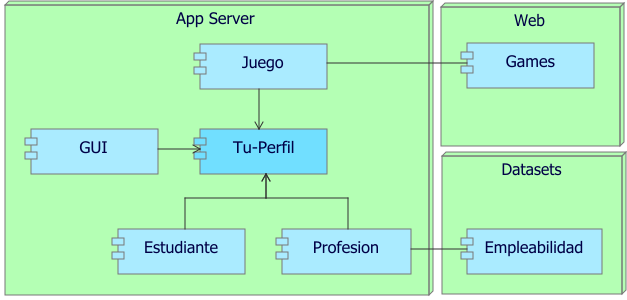
\includegraphics[width=.8\linewidth]{imgs/puntos_vista/tecnologia/uso.pdf}
	\caption{Caso de Uso de la Tecnología}
\end{figure}

Para nuestro caso, en el servidor de aplicaciones vamos a desplegar los componentes descritos en la capa de aplicación, a saber, el componente orquestador Tu-Perfil, los componentes pertenecientes al core de la aplicación, como lo son el componente Profesión, Juego, y Estudiante, además del componente del front, GUI. Por otra parte, se especifican dos componentes externos, el primero de ellos denominado Games, el cual, nos permite integrar juegos online que proporcionan datos sobre las partidas de los juegos y sus correspondientes puntajes en cada una de las modalidades o categorías para ser enviadas y analizadas para el perfilamiento del estudiante. Luego, se especifica el componente Empleabilidad, que nos brinda una estadística sobre las profesiones con mayor demanda en periodos de tiempo ajustables mediante el uso de diferentes datasets. 
\newpage
\section{Punto de Vista Estructura de Información}
Una estructura de información es una estructura jerárquica centrada en el producto que organiza la información relacionada con un producto o biblioteca. Dentro de una estructura de información, los subgrupos de información denominados grupos de información organizan el contenido. Estos objetos de contenido se denominan elementos de información. Los criterios de filtro ofrecen la posibilidad de identificar y administrar la información asociada a las variaciones del producto. Las estructuras de información se pueden filtrar para mostrar componentes opcionales o artículos con valores de atributo específicos. Los objetos se muestran en la estructura según el filtro de la estructura actualmente activo. Se pueden editar los filtros y renovar la estructura para mostrar los objetos que cumplen con los nuevos criterios de filtro. Las estructuras de información se pueden comparar para determinar el impacto de los cambios en el producto. La estructura de información que se encuentra actualmente en producción se puede comparar con una nueva estructura de información bajo desarrollo para revelar el impacto de los cambios propuestos. Las relaciones con la información de producto de soporte permiten determinar la cantidad y el ámbito del trabajo que se va a hacer.

\subsection{Modelo de Estructura de Información}
\begin{figure}[h!]
	\centering
	\includegraphics[width=.62\linewidth]{imgs/modelo/EstrInformacion}
	\caption{Modelo Estructura de Información}
\end{figure}

Esta quinta sección de puntos de vista llamada tecnología en la cual se involucra todo lo concerniente a la parte tecnológica, su uso, la implementación y el despliegue, la parte física, las capas, el servicio y la estructura de la información del proyecto, este último punto de vista de la estructura de información está compuesto por cinco elementos principalmente, tal y como se muestra en el diagrama anterior del modelo. Estos elementos son: como principal, está el objeto y el objeto secundario, luego se deriva en una representación y significado del mismo y por la parte de los objetos se desprende un artefacto por medio de una realización. 


\subsection{Caso  de Estructura de Información}
\begin{figure}[h!]
	\centering
	\includegraphics[width=.8\linewidth]{imgs/caso/estructuraInformaci}
	\caption{Caso Estructura de Información}
\end{figure}

El punto de vista de la estructura de la información es comparable a los modelos de información tradicionales creados en el desarrollo de casi cualquier sistema de información. Muestra la estructura de la información utilizada en la empresa o en un proceso de negocio o aplicación específicos, en términos de tipos de datos o estructuras de clases (orientadas a objetos). Además, puede mostrar cómo la información a nivel empresarial se representa en el nivel de la aplicación en la forma de las estructuras de datos que se utilizan allí, y cómo se asignan luego a la infraestructura tecnológica subyacente, destacando que es un enfoque de muy alto nivel hacia por ejemplo, por medio de un esquema de base de datos, tal y como se realizó para el proyecto Tu-Perfil en donde se tiene el objeto de negocio llamado Perfil Web y una serie de elementos o entidades importantes a tener en cuenta para modelar como los perfiles que tiene un perfil para una profesión y lógicamente el estudiante a perfilar, sin dejar de lado la parte del juego o Game que realiza la función de brochure para la base de datos.

\clearpage
\newpage
\section{Punto de Vista de Realización de Servicio}

Este punto de vista visualiza como por los procesos o componentes de aplicación se realizan los servicios de negocio, evidenciando el puente entre el punto de vista de producto del negocio y la vista de procesos del negocio. Como su nombre lo indica y se observa en el meta-modelo, en este punto de vista se deben identificar los elementos claves para realizar el servicio que ofrece la compañía, es
un tipo de resumen de los elementos generales y que se deben resaltar para comprender en su totalidad el servicio. En este punto de vista el elemento por el cual se debe iniciar el diseño, es el servicio de negocio, de él se derivan los procesos principales y los objetos de negocio asociados al
servicio; teniendo claro que los procesos de negocio se soportan con servicios de aplicación y componentes de aplicación, mientras que los objetos de negocio se realizan con objetos de aplicación. Los elementos que rodean los servicios, se utilizan para hacer claridad en los roles, actores y colaboraciones principales que intervienen en la realización de los procesos.

\subsection{Modelo de Realización de Servicio}
\begin{figure}[h!]
	\centering
	\includegraphics[width=1\linewidth]{imgs/modelo/RealServicio}
	\caption{Modelo Realización de Servicio}
\end{figure}

El punto de vista de realización del servicio muestra los procesos de negocio de la arquitectura: realización de la evaluación, consolidación de la información y análisis de resultados asignados a componentes de aplicación que serán de soporte para dichos proceso. Los procesos de negocio son realizados de forma secuencial y la realización de todos proveen los servicios de negocio definidos.

Este punto de vista cuenta con una gran y amplia serie de elementos que facilitan este proceso, iniciando por el actor en cuestión, con su rol y la colaboración que implica, posteriormente, se centra en el proceso servicio y evento que involucra, teniendo en cuenta también componentes e interfaces.


\subsection{Caso  de Realización de Servicio}
\begin{figure}[h!]
	\centering
	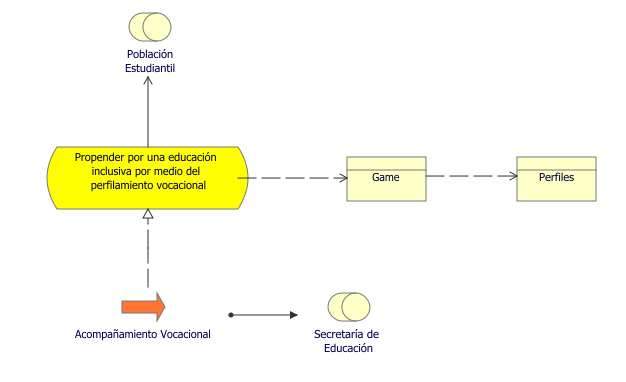
\includegraphics[width=1.05\linewidth]{imgs/caso/RealizaServicio}
	\caption{Caso Realización de Servicio}
\end{figure}

El punto de vista de realización de requerimientos de la parte tecnológica se realiza la vinculación de la información de la base de datos con los procesos de negocio, en busca de un ruta para abstraer nuevos elementos. En el caso del proyecto Tu-Perfil, se destaca el servicio principal de propender por una educación inclusiva por medio del perfilamiento vocacional que a su vez está dirigida al actor de la población estudiantil y a la secretaría de educación nacional a través del proceso de negocio principal llamado acompañamiento vocacional, posteriormente se encuentran los objetos Game o juego y el objeto de los Perfiles. De esta manera se construye el punto de vista de realización de servicio, teniendo en cuenta lo trabajado hasta el momento y dando bases para lo que sigue en la construcción del proyecto Tu-Perfil para la parte de la base de datos.
\newpage
\section{Punto de Vista Físico}
\subsection{Modelo Físico}
\begin{figure}[h!]
	\centering
	\includegraphics[width=.9\linewidth]{imgs/modelo/Fisico}
	\caption{Modelo Físico}
\end{figure}

El punto de vista físico es importante para los proyectos a realizar a escala industrial, no por el hecho de que sea fundamental para la construcción del proyecto sino más que todo es para su puesta en marcha. Como es bien sabido, todos los proyectos se realizan con alguna razón de ser, generalmente para cumplir una necesidad y/o ayudar a la comunidad con una función en específico, teniendo en cuenta esto, para la implementación y puesta en marcha del proyecto, es necesario tener en cuenta el punto de vista físico si el proyecto  así lo requiere.

Para el caso del proyecto Tu-Perfil, este no requiere un punto de vista físico como tal, puesto que no cuenta con los requisitos para que este exista, no se va a construir a gran escala o a escala industrial y todos los servicios que brinda este proyecto son digitales, por lo tanto aparte de las herramientas de computación y servidores no se requiere más indumentaria física.

\clearpage

\newpage
\section{Punto de Vista de Capas}

El punto de vista por capas muestra las diferentes capas y aspectos de la arquitectura empresarial en un modelo. Existen dos categorías de capas, capas dedicadas y capas de servicio. Las capas son resultado de la relación de “agrupación” para un particionado natural de todo el conjunto de objetos y relaciones que pertenecen al modelo. La infraestructura, la aplicación, los procesos y los actores/roles pertenecen a la primera categoría. El principio estructural es que cada capa dedicada expone por medio de una relación de “realización” una capa de servicios, las cuales serán “usadas por” la siguiente capa dedicadas. A partir de esto se puede separar la estructura interna y la organización de cada capa dedicada de su comportamiento externo observable expresado como el servicio que esa capa dedicada realiza. 

\subsection{Modelo de Capas}
\begin{figure}[h!]
	\centering
	\includegraphics[width=.5\linewidth]{imgs/modelo/Capas}
	\caption{Modelo de Capas}
\end{figure}

El modelo de capas muestra como los servicios de negocio, aplicación e infraestructura son integrados por medio de sus modelos intermedios: Se muestran los servicios de negocio principales y los procesos de negocio que los realizan, estos procesos están asociados con servicios de aplicación específicos que a su vez son realizados por componentes de aplicación definidos para la arquitectura del sistema de software. Los componentes se encuentran soportados en servicios de infraestructura realizados por nodos de infraestructura y aplicaciones de software concretas.


\subsection{Caso punto de vista de Capas}
\begin{figure}[h!]
	\centering
	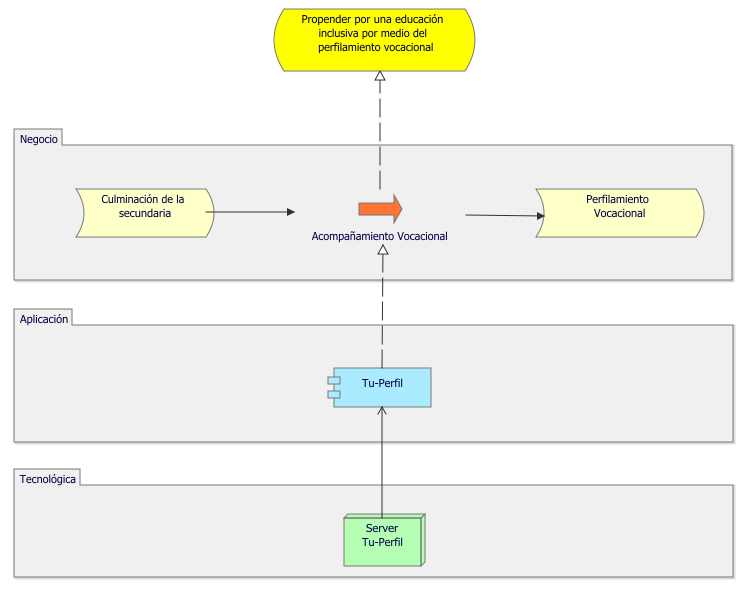
\includegraphics[width=1\linewidth]{imgs/caso/CapasTuPerfil}
	\caption{Caso de Capas}
\end{figure}

Para el caso del proyecto Tu-Perfil, el punto de vista de capas inicia con el objetivo central del proyecto Tu-Perfil, el cual es propender por una educación inclusiva por medio del perfilamiento vocacional y se conecta con tres capas fundamentales en el proceso de construcción del proyecto, estas capas son: la capa de negocio en la cual se especifica lo más relevante trabajado en esos puntos de vista pertenencientes a la capa de negocio contando con el proceso principal del acompañamiento vocacional precedido por la culminación de la secundaria y lo sucede el perfilamiento vocacional. Sigue la capa de aplicación con el paquete principal de Tu-Perfil y la capa tecnológica con el servidor Tu-Perfil.

\clearpage